\documentclass[RNAAS,linenumbers]{aastex631}
\usepackage{amsmath}
\newcommand{\tess}{\textit{TESS}}

\begin{document}

\title{Three Transiting Candidates around Faint M Dwarfs from an Agent-Driven Search of \tess\ Full-Frame Images}

\author{Kishore Hariharan}
\affiliation{Generative Experiences, Orlando, FL, USA}
\email{company@genexperiences.com}

\keywords{Exoplanet detection methods (489) --- Transit photometry (1709) --- M dwarf stars (982) --- Astronomy software (1855)}

\begin{abstract}
We report three transiting planet candidates around M dwarfs with \tess\ magnitudes 13.8--14.8, identified in an independent box-least-squares search of SPOC full-frame image (FFI) cutouts of 38,620 Sector 1 stars with $12<T<15$ and $R_\star<0.6\,R_\odot$ that were neither 2-minute targets nor \tess\ Objects of Interest. Each signal is recovered independently in every available sector (3--9 sectors, 2018--2026), is located on the target in noise-normalized difference images, shows consistent odd and even depths and no secondary eclipse, and is fit with a physical transit model. TIC~389723320 hosts a $4.6\,R_\oplus$ candidate at $P=3.927167$~d; TIC~114949540 a $4.35\,R_\oplus$ candidate at $P=2.739176$~d; and TIC~259719966 a $0.94\,R_{\rm Jup}$ companion at $P=11.077205$~d whose nature requires a mass measurement. None appears in the TOI, Community Candidate, or confirmed-planet lists. The pipeline was built and operated with an AI coding agent under human direction; code and per-candidate vetting reports are public.
\end{abstract}

\section{Motivation}
The \tess\ project's own FFI transit searches have concentrated on stars brighter than $T\approx13.5$ \citep{huang2020,kunimoto2022}, leaving the fainter M-dwarf population, where a given planet produces the deepest transits, comparatively under-searched. We targeted that population directly: M dwarfs ($T_{\rm eff}<4000$~K, $R_\star<0.6\,R_\odot$) with $12<T<15$, excluding 2-minute targets, TOIs, Community Candidates, and known planet hosts. For Sector 1 this yields 40,328 unique stars, of which the 38,620 with contamination ratio below 1 were searched.

\section{Data and Search}
For each star we extracted a $15\times15$ pixel cutout from the SPOC calibrated FFI sector cubes hosted on AWS \citep[astrocut;][]{brasseur2019}, defined a threshold aperture, summed the aperture flux, and removed shared systematics by regressing against the leading principal components of the non-aperture pixels \citep[lightkurve;][]{lightkurve2018}. After normalization, a 33-hour Savitzky--Golay flatten, and a point-to-point-jump filter for pointing excursions, we ran a box least squares search \citep{kovacs2002} over 0.3--13~d with durations 0.5--6~h. Candidates required S/N~$\geq9$, depth $\geq3000$~ppm, at least two transits, duration no more than $1.5\times$ the maximum allowed by the TIC stellar density \citep{stassun2019}, duty cycle below 15\%, odd and even depths consistent within $3\sigma$, and no secondary eclipse at phase 0.5 above $3\sigma$. Twenty-two stars passed.

\section{Vetting}
Each flagged star was tested against Gaia DR3 \citep{gaia2023} neighbors within 2 pixels, with the eclipse depth each neighbor would need to reproduce the signal; a flux-weighted centroid shift between in- and out-of-transit cadences; and a difference image (out-of-transit mean minus in-transit mean, per-frame plane-subtracted, divided by its per-pixel noise) whose peak locates the source of the dip \citep{bryson2013,twicken2018}. Of the 22, seven were located on a neighbor, one was a spotted rotator, one an unresolvable 1\arcsec\ blend, and three showed anomalous centroid behavior. Every survivor was then searched independently in each sector in which \tess\ observed it \citep[sectors from tess-point;][]{burke2020} and the sectors stitched to refine the period. Two high-S/N single-sector detections failed to repeat and were dropped. Three candidates passed all tests.

\section{Candidates}
Transit parameters were obtained with \texttt{batman} \citep{kreidberg2015} and \texttt{emcee} \citep{foremanmackey2013}, fitting epoch, period, $R_p/R_\star$, $a/R_\star$, impact parameter, and quadratic limb darkening with Gaussian priors ($0.3\pm0.1$), super-sampling each sector to its exposure time. Stellar parameters are from TIC v8. Figure~\ref{fig:folds} shows the phase-folded data and models.

\textbf{TIC 389723320} ($T=14.52$, $T_{\rm eff}=3271$~K, $R_\star=0.37\,R_\odot$, $d=126$~pc). Six sectors (1, 28, 68, 95, 105, 106), 36 transits. $P=3.927167\pm0.000001$~d, $T_0=2460899.3895\pm0.0005$ BJD, depth $12{,}850\pm690$~ppm, duration $1.50\pm0.06$~h, $b=0.74$, $R_p=4.62\pm0.13\,R_\oplus$, $T_{\rm eq}\approx565$~K. Odd minus even depth $1100\pm520$~ppm ($2.1\sigma$). Difference images in sectors 68, 95, and 105 peak on the target at 14, 14, and 18$\sigma$. Transit-derived stellar density $4.1^{+1.5}_{-1.0}\,\rho_\odot$ versus 7.0 from the TIC, consistent within the $b$--$a/R_\star$ degeneracy.

\textbf{TIC 114949540} ($T=14.78$, $T_{\rm eff}=3320$~K, $R_\star=0.42\,R_\odot$, $d=168$~pc). Three sectors (1, 27, 105), 25 transits. $P=2.739176\pm0.000001$~d, $T_0=2461212.9505\pm0.0007$ BJD, depth $8930\pm710$~ppm, duration $1.55\pm0.07$~h, $b=0.53$, $R_p=4.35\pm0.17\,R_\oplus$, $T_{\rm eq}\approx670$~K. Odd minus even $-240\pm450$~ppm. Difference images in sectors 27 and 105 peak on the target at 15 and 8$\sigma$.

\textbf{TIC 259719966} ($T=13.80$, $T_{\rm eff}=3443$~K, $R_\star=0.49\,R_\odot$, $d=147$~pc). Nine sectors (1, 27, 67, 94, 95, 101--104), 20 transits. $P=11.077205\pm0.000001$~d, $T_0=2460877.8231\pm0.0002$ BJD, depth $38{,}300\pm1200$~ppm (undiluted sectors), duration $2.37\pm0.03$~h, $b=0.55$, $R_p=10.58\pm0.17\,R_\oplus$ ($0.94\,R_{\rm Jup}$), $T_{\rm eq}\approx400$~K. Odd minus even $-230\pm370$~ppm; secondary $20\pm540$~ppm. Difference images in sectors 94 and 104 peak on the target at 33 and 37$\sigma$. A Gaia neighbor 2.1~px away (27\% of the target's $G$-band flux) enters the automatic aperture in three sectors and dilutes the depth there; the sense of that effect (shallower when included) independently places the dip on the target. With a radius near Jupiter's, the companion may be a giant planet, a brown dwarf, or a star near the hydrogen-burning limit; its radial-velocity semi-amplitude would exceed 100~m~s$^{-1}$ for any stellar-mass companion.

A residual search of the stitched light curves of the first two systems, with the known transits masked, found no additional signal above $\sim$1000~ppm with three or more transits at $P<30$~d.

\begin{figure}[ht!]
\centering
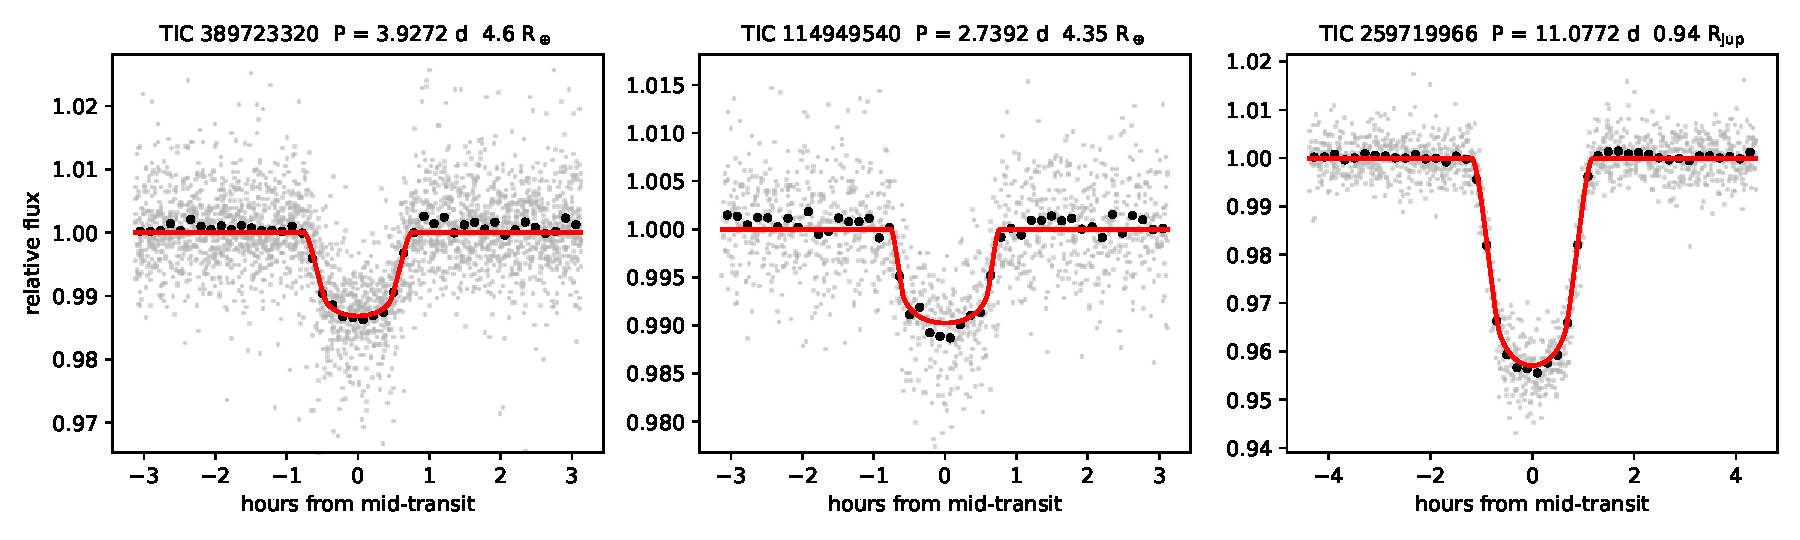
\includegraphics[width=\textwidth]{figure1.pdf}
\caption{Phase-folded \tess\ FFI photometry (all sectors, gray) with the posterior-median transit model (red) for TIC~389723320 (left), TIC~114949540 (center), and TIC~259719966 (right). Binned points in black.}
\label{fig:folds}
\end{figure}

\section{Caveats and Availability}
All three hosts are faint for radial-velocity follow-up; TIC~259719966 is the most tractable. None of the candidates is a TOI, Community Candidate (ExoFOP list of 2026 October 24), or known planet host; none has an ADS literature match; and none lies within 30\arcsec\ of an entry in the DIAmante FFI candidate catalog \citep{montalto2020}, the QLP faint-star TOI release \citep{kunimoto2022}, the \tess\ eclipsing binary catalog \citep{prsa2022}, or the Gaia DR3 variability classification. The pipeline (target selection, parallel FFI sweep, vetting, multi-sector recovery, MCMC fitting, and report generation) was written and operated with Claude, an AI coding agent, directed by the author, who has no prior background in exoplanet science; we note this because the result bears on how such searches can be scaled. Code, pitfalls log, and per-candidate vetting reports are available at \url{https://github.com/khariha/tess-hunt}.

\begin{acknowledgments}
This research made use of data from the \tess\ mission, obtained from MAST at STScI. The \tess\ full-frame images used here can be found in MAST: \dataset[10.17909/t9-17nt-6c71]{https://doi.org/10.17909/t9-17nt-6c71}. It made use of the NASA Exoplanet Archive \dataset[10.26133/NEA12]{https://doi.org/10.26133/NEA12} and ExoFOP \dataset[10.26134/ExoFOP5]{https://doi.org/10.26134/ExoFOP5}, operated by Caltech/IPAC under contract with NASA, and of data from the ESA mission Gaia, processed by the Gaia DPAC.
\end{acknowledgments}

\software{astrocut \citep{brasseur2019}, astropy, astroquery, batman \citep{kreidberg2015}, emcee \citep{foremanmackey2013}, lightkurve \citep{lightkurve2018}, tess-point \citep{burke2020}, Modal}

\begin{thebibliography}{}
\bibitem[Brasseur et al.(2019)]{brasseur2019} Brasseur, C. E., Phillip, C., Fleming, S. W., Mullally, S. E., \& White, R. L. 2019, Astrocut: Tools for creating cutouts of TESS images, Astrophysics Source Code Library, ascl:1905.007
\bibitem[Bryson et al.(2013)]{bryson2013} Bryson, S. T., Jenkins, J. M., Gilliland, R. L., et al. 2013, PASP, 125, 889
\bibitem[Burke et al.(2020)]{burke2020} Burke, C. J., Levine, A., Fausnaugh, M., et al. 2020, TESS-Point: High precision TESS pointing tool, Astrophysics Source Code Library, ascl:2003.001
\bibitem[Foreman-Mackey et al.(2013)]{foremanmackey2013} Foreman-Mackey, D., Hogg, D. W., Lang, D., \& Goodman, J. 2013, PASP, 125, 306
\bibitem[Gaia Collaboration et al.(2023)]{gaia2023} Gaia Collaboration, Vallenari, A., Brown, A. G. A., et al. 2023, A\&A, 674, A1
\bibitem[Huang et al.(2020)]{huang2020} Huang, C. X., Vanderburg, A., P\'al, A., et al. 2020, RNAAS, 4, 204
\bibitem[Kov\'acs et al.(2002)]{kovacs2002} Kov\'acs, G., Zucker, S., \& Mazeh, T. 2002, A\&A, 391, 369
\bibitem[Kreidberg(2015)]{kreidberg2015} Kreidberg, L. 2015, PASP, 127, 1161
\bibitem[Kunimoto et al.(2022)]{kunimoto2022} Kunimoto, M., Daylan, T., Guerrero, N., et al. 2022, ApJS, 259, 33
\bibitem[Lightkurve Collaboration et al.(2018)]{lightkurve2018} Lightkurve Collaboration, Cardoso, J. V. d. M., Hedges, C., et al. 2018, Lightkurve: Kepler and TESS time series analysis in Python, Astrophysics Source Code Library, ascl:1812.013
\bibitem[Montalto et al.(2020)]{montalto2020} Montalto, M., Borsato, L., Granata, V., et al. 2020, MNRAS, 498, 1726
\bibitem[Pr\v{s}a et al.(2022)]{prsa2022} Pr\v{s}a, A., Kochoska, A., Conroy, K. E., et al. 2022, ApJS, 258, 16
\bibitem[Stassun et al.(2019)]{stassun2019} Stassun, K. G., Oelkers, R. J., Paegert, M., et al. 2019, AJ, 158, 138
\bibitem[Twicken et al.(2018)]{twicken2018} Twicken, J. D., Catanzarite, J. H., Clarke, B. D., et al. 2018, PASP, 130, 064502
\end{thebibliography}

\end{document}
